\documentclass[10pt,a4paper]{article}
\usepackage[utf8]{inputenc}
\usepackage{amsmath}
\usepackage{amsfonts}
\usepackage[margin=1in]{geometry}
\usepackage{amssymb}
\usepackage{tikz}
\author{Joel Mizzoni (jmizzoni), Patrick White (ps2white)}
\begin{document}
\title{ECE358 S'16 Assignment 4}
\maketitle
\section{}
Here we answer question 1
\section{}
Here we answer question 2
\section{}
Here we answer question 3
\section{}
Here we answer question four
\section{}
Here we answer question 5
\section{}
Here we answer question 6
\section{}
A network that would cause this to occur looks like this:

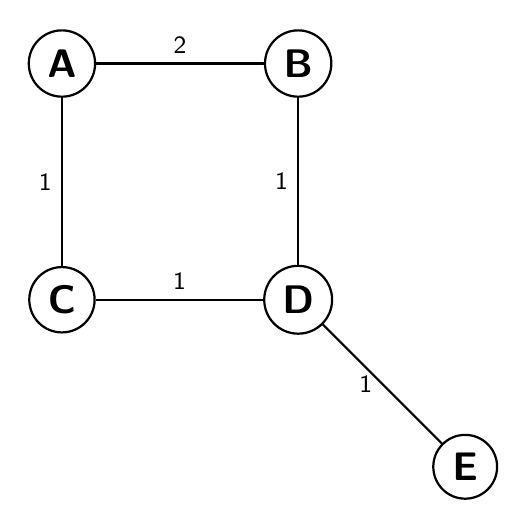
\begin{tikzpicture} [auto, node distance=3cm, every loop/.style={},
                    thick,main node/.style={circle,draw,font=\sffamily\Large\bfseries}]
    \node[main node] (1){A};
    \node[main node] (2)[right of=1]{B};
    \node[main node] (3)[below of=1]{C};
    \node[main node] (4)[below of=2]{D};
    \node[main node] (5)[below right of=4]{E};

    \path[every node/.style={font=\sffamily\small}]
    (1) edge node [above] {2} (2)
        edge node [left] {1} (3)
    (2) edge node [left] {1} (4)
    (3) edge node [above] {1} (4)
    (4) edge node [left] {1} (5);
\end{tikzpicture}
If the cost from $D \leftrightarrow E$ is updated to some large value (e.g. 50), assume that D notices the change first.
The first update will result in D routing through C to get to E (assuming a path cost of 3). D then broadcasts the update to B and C.
Assume C receives the update first. Using poisoned reverse, C will choose to route to E through A (cost 4). 
A will then choose to route through B (cost 4), and then B will still think it can route through D with a cost of 2.
At this point, before the other updates are processed, the loop has started, and a packet will travel from $A \rightarrow C \rightarrow D \rightarrow B \rightarrow A \ldots$ until the routing tables converge to taking the path from D to E.

\end{document}
